\documentclass{article}\usepackage[]{graphicx}\usepackage[]{color}
%% maxwidth is the original width if it is less than linewidth
%% otherwise use linewidth (to make sure the graphics do not exceed the margin)
\makeatletter
\def\maxwidth{ %
  \ifdim\Gin@nat@width>\linewidth
    \linewidth
  \else
    \Gin@nat@width
  \fi
}
\makeatother

\definecolor{fgcolor}{rgb}{0.345, 0.345, 0.345}
\newcommand{\hlnum}[1]{\textcolor[rgb]{0.686,0.059,0.569}{#1}}%
\newcommand{\hlstr}[1]{\textcolor[rgb]{0.192,0.494,0.8}{#1}}%
\newcommand{\hlcom}[1]{\textcolor[rgb]{0.678,0.584,0.686}{\textit{#1}}}%
\newcommand{\hlopt}[1]{\textcolor[rgb]{0,0,0}{#1}}%
\newcommand{\hlstd}[1]{\textcolor[rgb]{0.345,0.345,0.345}{#1}}%
\newcommand{\hlkwa}[1]{\textcolor[rgb]{0.161,0.373,0.58}{\textbf{#1}}}%
\newcommand{\hlkwb}[1]{\textcolor[rgb]{0.69,0.353,0.396}{#1}}%
\newcommand{\hlkwc}[1]{\textcolor[rgb]{0.333,0.667,0.333}{#1}}%
\newcommand{\hlkwd}[1]{\textcolor[rgb]{0.737,0.353,0.396}{\textbf{#1}}}%
\let\hlipl\hlkwb

\usepackage{framed}
\makeatletter
\newenvironment{kframe}{%
 \def\at@end@of@kframe{}%
 \ifinner\ifhmode%
  \def\at@end@of@kframe{\end{minipage}}%
  \begin{minipage}{\columnwidth}%
 \fi\fi%
 \def\FrameCommand##1{\hskip\@totalleftmargin \hskip-\fboxsep
 \colorbox{shadecolor}{##1}\hskip-\fboxsep
     % There is no \\@totalrightmargin, so:
     \hskip-\linewidth \hskip-\@totalleftmargin \hskip\columnwidth}%
 \MakeFramed {\advance\hsize-\width
   \@totalleftmargin\z@ \linewidth\hsize
   \@setminipage}}%
 {\par\unskip\endMakeFramed%
 \at@end@of@kframe}
\makeatother

\definecolor{shadecolor}{rgb}{.97, .97, .97}
\definecolor{messagecolor}{rgb}{0, 0, 0}
\definecolor{warningcolor}{rgb}{1, 0, 1}
\definecolor{errorcolor}{rgb}{1, 0, 0}
\newenvironment{knitrout}{}{} % an empty environment to be redefined in TeX

\usepackage{alltt}
\usepackage[ngerman]{babel}

\title{Results of modified Bland Altman analysis}
\author{Inga Könemund}
\date{\today}
\IfFileExists{upquote.sty}{\usepackage{upquote}}{}
\begin{document}

\maketitle

\newpage
\section{Analysis results}

% include analysis results as table




% latex table generated in R 3.5.2 by xtable 1.8-3 package
% Wed Mar 06 12:28:17 2019
\begin{table}[ht]
\centering
\begin{tabular}{rrrr}
  \hline
 & value &   & +/- SE \\ 
  \hline
Bias & 0.4976740 &  &  \\ 
  SD of the differences & 0.8229147 &  &  \\ 
  lower limit of agreement & -1.1152388 &  &  \\ 
  upper limit of agreement & 2.1105868 &  &  \\ 
  MOVER CI lower LoA & -1.4267447 & -0.8041530 &  \\ 
  MOVER CI upper LoA & 1.7995010 & 2.4220927 &  \\ 
  BA CI lower LoA & -1.6141143 & -0.6163633 &  \\ 
  BA CI upper LoA & 1.6117113 & 2.6094623 &  \\ 
  Within-subject variance (WSV) & 0.1861722 &  &  \\ 
  Between-subject variance (BSV) & 0.4910164 &  &  \\ 
   \hline
\end{tabular}
\end{table}


% include analysis results as plot



\begin{knitrout}
\definecolor{shadecolor}{rgb}{0.969, 0.969, 0.969}\color{fgcolor}
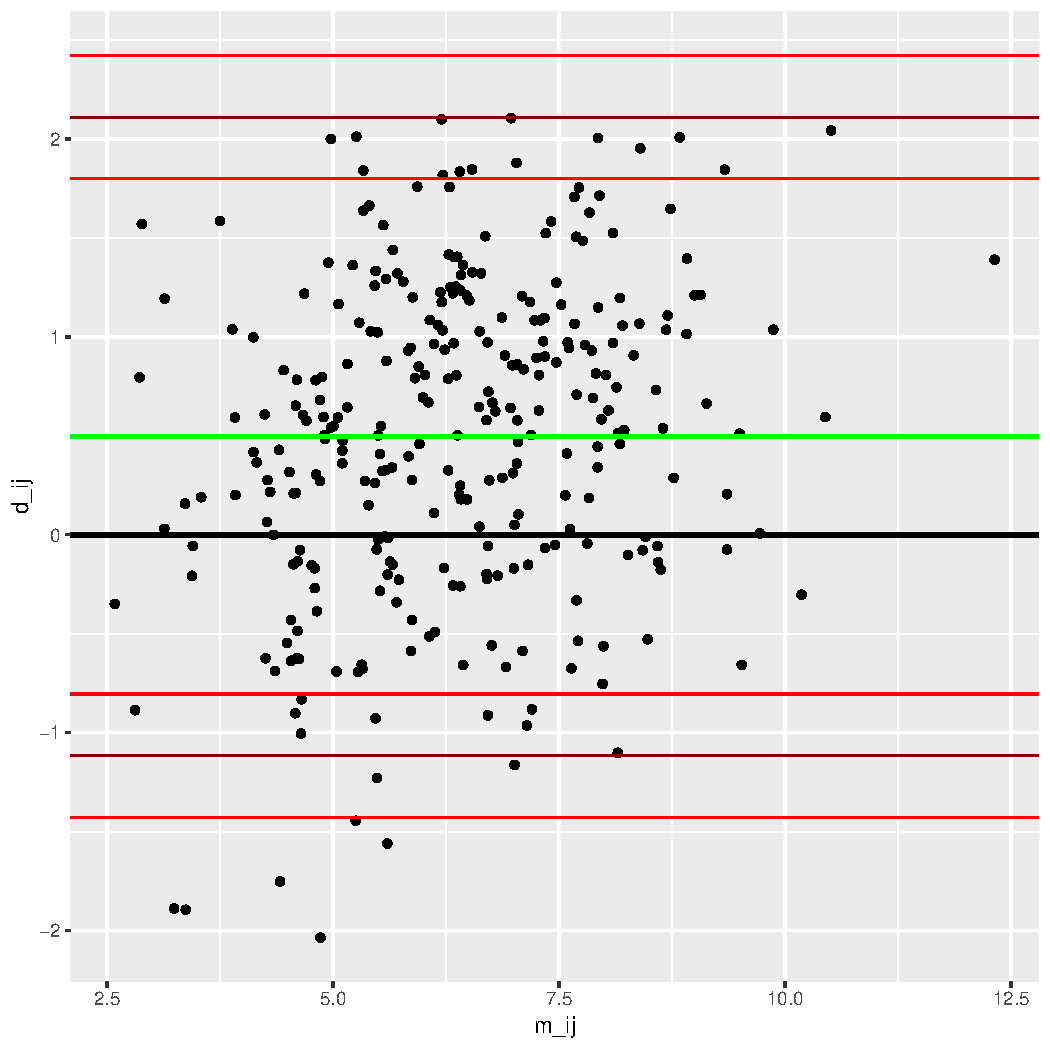
\includegraphics[width=\maxwidth]{figure/analysisResults_plot-1} 

\end{knitrout}

\section{Table of the individual means}





% latex table generated in R 3.5.2 by xtable 1.8-3 package
% Wed Mar 06 12:28:19 2019
\begin{table}[ht]
\centering
\begin{tabular}{rrr}
  \hline
subject & Mean & M \\ 
  \hline
       1 & 0.8786727 &       15 \\ 
         2 & 0.1697973 &       15 \\ 
         3 & -1.2579040 &       15 \\ 
         4 & 0.0944813 &       15 \\ 
         5 & 1.1625367 &       15 \\ 
         6 & -0.2139313 &       15 \\ 
         7 & 1.4141673 &       15 \\ 
         8 & 1.3310160 &       15 \\ 
         9 & 0.1084060 &       15 \\ 
        10 & 0.8762600 &       15 \\ 
        11 & 0.7456387 &       15 \\ 
        12 & 0.4427293 &       15 \\ 
        13 & -0.3051773 &       15 \\ 
        14 & 0.9632920 &       15 \\ 
        15 & 0.2107773 &       15 \\ 
        16 & 1.0315840 &       15 \\ 
        17 & 1.1759320 &       15 \\ 
        18 & 1.2249780 &       15 \\ 
        19 & -0.5016893 &       15 \\ 
        20 & 0.4019133 &       15 \\ 
   \hline
\end{tabular}
\end{table}


\end {document}
